\documentclass[11pt, a4paper]{csiroreport2012}

\usepackage{graphicx}
\usepackage{amssymb}
\usepackage{amsmath}
\usepackage{booktabs}
\usepackage[small]{caption}
\usepackage[authoryear]{natbib}
\usepackage{authblk}
\usepackage{framed}
\definecolor{shadecolor}{gray}{0.9}




\setlength{\belowcaptionskip}{\abovecaptionskip} % Space below table caption same as that above
									      % figure caption
\docdivision[ENERGY FLAGSHIP]
\doctitle[{\huge NUMBAT} \\ High-resolution simulations of density-driven convective mixing\\User manual]
\docauthors[\vspace{1cm} Christopher P.  Green and Jonathan Ennis-King]
\docreportnum[Report Number ****]
\docreportdate[\today]
\doccopyrightyear[2015]

\docfootertitle[Numbat user manual]

\docbusinessunit[CSIRO Energy Flagship \\
71 Normanby Road, Clayton VIC, 3168, Australia \\
Private Bag 10, Clayton South VIC, 3169, Australia \\
Telephone: +61 3 9545 2777 \\
Fax: +61 3 9545 8380]

\docfurtherinfoA[CSIRO Energy Flagship]{Chris Green}
{+61 3 9545 8371}{chris.green@csiro.au}{}{www.csiro.au}

\begin{document}

\section{Introduction}

Numbat is a finite element application for solving the coupled Darcy and convection-diffusion equations for density-driven convective mixing in porous media. Numbat is built on the MOOSE Framework (www.mooseframework.com), and leverages multiple powerful features from this foundation. It features mesh adaptivity, high-order finite elements, is massively parallel, and uses a simple plain text input file. 

\section{Theory}

A simple illustration of the problem under consideration is presented in Figure \ref{fig:schematic} for a two-dimensional representation. In this case, we have a 
\begin{figure}[ht]
\begin{center}
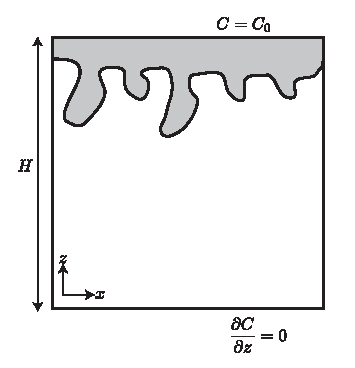
\includegraphics[width=100mm]{figures/schematic.pdf}
\caption{Schematic of 2D model. No-flow boundary conditions are imposed at the bottom boundary, and periodic boundary conditions are applied along the lateral boundaries. A constant concentration boundary condition is applied at the top boundary.}
\label{fig:schematic}
\end{center}
\end{figure}

The governing equations for density-driven flow in porous media are Darcy's law
\begin{equation}
\mathbf{u} = - \frac{\mathbf{K}}{\mu} \left(\nabla P + \rho(c) g \hat{\mathbf{k}} \right),
\label{eq:darcy}
\end{equation}
where $\mathbf{u} = (u, v, w)$ is the velocity vector, $\mathbf{K}$ is permeability, $\mu$ is the fluid viscosity, $P$ is the fluid pressure, $\rho(c)$ is the fluid density as a function of solute concentration $c$, $g$ is gravity, and $\hat{\mathbf{k}}$ is the unit vector in the $z$ direction.

The fluid velocity must also satisfy the continuity equation
\begin{equation}
\nabla \cdot \mathbf{u} = 0,
\end{equation}
and the solute concentration is governed by the convection - diffusion equation
\begin{equation}
\phi \frac{\partial c}{\partial t} + \mathbf{u} \cdot \nabla c = \phi D \nabla^2 c,
\label{eq:convdiff}
\end{equation}
where $\phi$ is the porosity, $t$ is time and $D$ is the diffusivity. 

Darcy's law and the convection-diffusion equations are coupled through the fluid density, which is given by
\begin{equation}
\rho(c) = \rho_0 + \frac{c}{c_0} \Delta \rho,
\label{eq:density}
\end{equation}
where $c_0$ is the equilibrium concentration, and $\Delta \rho$ is the increase in density of the fluid at equilibrium concentration.

The boundary conditions are
\begin{align}
w = 0,&  \quad z = 0, -H, \\
\frac{\partial c}{\partial z} = 0,& \quad z = -H, \\
c = c_0,& \quad z = 0,
\end{align}
which correspond to impermeable boundary conditions at the top and bottom boundaries ($z = 0$ and $z=-H$, respectively), and a saturated condition at the top boundary.

Initially, there is no solute in the model
\begin{equation}
c = 0, \quad t = 0.
\end{equation}

The solution of the governing equations differs in 2D and 3D. As a result, we shall consider the two cases separately. 

\subsection{2D model}

If we consider an anisotropic model, with vertical and horizontal permeabilities given by $k_z$ and $k_x$, respectively, we can non-dimensionalise the governing equations in 2D following \cite{EnnisKing2005}. Defining the anisotropy ratio $\gamma$ as
\begin{equation}
\gamma = \frac{k_z}{k_x},
\label{eq:gamma}
\end{equation}
we scale the variables using
\begin{align}
x = \frac{\phi \mu D}{k_z \Delta \rho g \gamma^{1/2}} \hat{x}, \quad z =  \frac{\phi \mu D}{k_z \Delta \rho g} \hat{z}, \quad u = \frac{k_z \Delta \rho g}{\mu \gamma^{1/2}} \hat{u}, \quad w = \frac{k_z \Delta \rho g}{\mu} \hat{w} \nonumber \\
t = \left(\frac{\phi \mu}{k_z \Delta \rho g}\right)^2 \hat{t}, \quad c = c_0 \hat{c}, \quad P = \frac{\mu \phi D}{k_z}\hat{P}, \qquad \qquad \qquad
\label{eq:scales}
\end{align}
where $\hat{x}$ refers to a dimensionless variable. The governing equations in dimensionless form are then
\begin{align}
\mathbf{u} = & - \left(\nabla P + c \mathbf{\hat{k}}\right), \label{eq:darcydim}\\
\mathbf{u} = & \,0, \label{eq:ctydim} \\
\frac{\partial c}{\partial t} + \mathbf{u} \cdot \nabla c = &\,  \gamma \frac{\partial^2 c}{\partial x^2} + \frac{\partial^2 c}{\partial z^2}, \label{eq:condiffdim}
\end{align}
where we have dropped the hat on the dimensionless variables for brevity.

The dimensionless boundary conditions are
\begin{align}
w = 0,&  \quad z = 0, -Ra, \label{eq:dimbc1} \\
\frac{\partial c}{\partial z} = 0,& \quad z = -Ra, \label{eq:dimbc2}\\
c = 1,& \quad z = 0, \label{eq:dimbc3}
\end{align}
where $Ra$ is the Rayleigh number, defined as
\begin{equation}
Ra = \frac{k_z \Delta \rho g H}{\phi \mu D}.
\label{eq:ra}
\end{equation}

In this form, the Rayleigh number only appears in the boundary conditions as the location of the lower boundary. Therefore, $Ra$ can be interpreted in this formalism as a dimensionless model height, and can be varied in simulations by simply changing the height of the mesh.

Finally, the dimensionless initial condition is
\begin{equation}
c = 0, \quad t = 0.
\label{eq:ic}
\end{equation}

For isotropic models, where $k_x = k_z$ and hence $\gamma = 1$, we recover the dimensionless equations given by \cite{Slim2014}.

The coupled governing equations must be solved numerically. To simplify the numerical analysis, we introduce the streamfunction $\psi(x,z,t)$ such that
\begin{equation}
u = - \frac{\partial \psi}{\partial z}, \quad w = \frac{\partial \psi}{\partial x}.
\label{eq:2Dstreamfunction}
\end{equation}
This definition satisfies the continuity equation, Eq.~(\ref{eq:ctydim}), immediately. 

The pressure $P$ is removed from Eq.~(\ref{eq:darcydim}) by taking the curl of both sides and noting that $\nabla \times \nabla P = 0 $ for any $P$, to give
\begin{equation}
\nabla^2 \psi = - \frac{\partial c}{\partial x},
\label{eq:darcypsi}
\end{equation}
where we have introduced the streamfunction $\psi$ using Eq.~(\ref{eq:2Dstreamfunction}).

The convection-diffusion equation, Eq.~(\ref{eq:condiffdim}) becomes
\begin{equation}\frac{\partial c}{\partial t} - \frac{\partial \psi}{\partial z} \frac{\partial c}{\partial x} + \frac{\partial \psi}{\partial x} \frac{\partial c}{\partial z} = \gamma \frac{\partial^2 c}{\partial x^2} + \frac{\partial^2 c}{\partial z}.
\label{eq:condiffpsi}
\end{equation}

The boundary conditions become
\begin{align}
\frac{\partial \psi}{\partial x} = 0,&  \quad z = 0, -Ra, \\
\frac{\partial c}{\partial z} = 0,& \quad z = -Ra, \\
c = 1,& \quad z = 0,
\label{eq:bcpsi}
\end{align}
while the initial condition is still given by Eq.~(\ref{eq:ic}).

In two dimensions, Numbat solves Eq's.~(\ref{eq:darcypsi}) and (\ref{eq:condiffpsi}) using the finite element method.

\subsection{3D model}

We now consider the case of a three-dimensional model. For simplicity, we consider the case where all lateral permeabilities are equal ($k_y = k_x$). The governing equations for the 3D model are identical to the 2D model. In dimensionless form, they are given by Eq's.~(\ref{eq:darcydim}) to (\ref{eq:condiffdim}), with boundary conditions given by Eq's.~(\ref{eq:dimbc1}) to (\ref{eq:dimbc3}), and initial condition given by Eq.~(\ref{eq:ic}).

To solve these governing equations in 3D, a different approach must be used as the streamfunction $\psi$ is not defined in three dimensions. Instead, we define a vector potential $\Psi = (\psi_x, \psi_y, \psi_z)$ such that
\begin{equation}
\mathbf{u} = \nabla \times \Psi.
\label{eq:Psi}
\end{equation}

It is important to note that the vector potential is only known up to the addition of the gradient of a scalar $\zeta$, since 
\begin{equation}
\nabla \times \left( \Psi + \nabla \zeta \right) = \nabla \times \Psi,
\end{equation}
as $\nabla \times \nabla \zeta = 0$ for any scalar $\zeta$. This uncertainty is referred to as guage freedom, and is common in electrodynamics. Taking the curl of Eq.~(\ref{eq:darcydim}) and substituting Eq.~(\ref{eq:Psi}), we have 
\begin{equation}
\nabla(\nabla \cdot \Psi) - \nabla^2 \Psi = \left(\frac{\partial c}{\partial y}, - \frac{\partial c}{\partial x}, 0\right),
\end{equation}
where we have again used the fact that $\nabla \times \nabla P = 0$. If we choose $\nabla \cdot \Psi = 0$ to specify the guage condition, this simplifies to
\begin{equation}
\nabla^2 \Psi = \left(-\frac{\partial c}{\partial y},  \frac{\partial c}{\partial x}, 0\right).
\label{eq:poisson}
\end{equation}

As shown in \cite{E1997}, $\nabla \cdot \Psi = 0$ is satisfied throughout the domain if 
\begin{align}
\psi_x = \psi_y = 0,& \quad z = 0, -Ra, \nonumber \\
\frac{\partial \psi_z}{\partial z} = 0, & \quad  z = 0, -Ra.
\end{align}

The governing equations are then 
\begin{align}
\nabla^2 \Psi = \,& \left(-\frac{\partial c}{\partial y}, \frac{\partial c}{\partial x}, 0 \right), \label{eq:darcy3d} \\
\frac{\partial c}{\partial t} + \mathbf{u} \cdot \nabla c = \, & \gamma \left( \frac{\partial^2 c}{\partial x^2} + \frac{\partial^2 c}{\partial y^2} \right) + \frac{\partial^2 c}{\partial z^2}, \label{eq:convdiff3d}
\end{align}
where the continuity is satisfied automatically because $\nabla \cdot \left( \nabla \times \Psi \right) = 0$ for any $\Psi$.

Finally, it is straightforward to show that $\psi_z = 0$ in order to satisfy $\nabla^2 \psi_z = 0$ and $\frac{\partial \psi_z}{\partial z} = 0$, which means that the vector potential has only $x$ and $y$ components, 
\begin{equation}
\Psi = (\psi_x, \psi_y, 0),
\end{equation}
and therefore the fluid velocity $\mathbf{u} = (u, v, w)$ is
\begin{equation}
\mathbf{u} = \left( -\frac{\partial \psi_y}{\partial z}, \frac{\partial \psi_x}{\partial z}, \frac{\partial \psi_y}{\partial x} - \frac{\partial \psi_x}{\partial y} \right).
\end{equation}

Note that if there is no $y$ dependence, Eq's.~(\ref{eq:darcy3d}) and (\ref{eq:convdiff3d}) reduce to 
\begin{align}
\nabla^2 \Psi = \, & \left(0, \frac{\partial c}{\partial x}, 0 \right), \\
\frac{\partial c}{\partial t} + \mathbf{u} \cdot \nabla c = \, & \gamma \frac{\partial^2 c}{\partial x^2}  + \frac{\partial^2 c}{\partial z^2}.
\end{align}
It is simple to show that $\nabla^2 \psi_x = 0$ and $\psi_x = 0$ at $z = 0, -Ra$ are only satisfied if $\psi_x = 0$ in the entire domain. In this case, the governing equations reduce to the two-dimensional formulation, as expected.

In three dimensions, Numbat solves Eq's.~(\ref{eq:darcy3d}) and (\ref{eq:convdiff3d}) using the finite element method.

%% Installation
\section{Installation}



\subsubsection*{Install MOOSE}
 Numbat is  a MOOSE application. In order to run Numbat, the MOOSE framework must first be installed. Detailed instructions are available at www.mooseframework.com/getting-started.
 
 \subsubsection*{Clone Numbat}
 
 The next step is to clone Numbat from GitHub. In the following, it assumed that MOOSE was installed to the directory \texttt{$\sim$/projects}. If MOOSE was installed to a different directory, the following instructions must be modified accordingly.

To clone Numbat, use the following commands at the command line:

\begin{verbatim}
cd ~/projects
git clone https://github.com/cpgr/numbat.git
cd numbat
git checkout master
\end{verbatim}

At this stage, there should be a \texttt{$\sim$/projects/numbat} directory.

\subsubsection*{Compile Numbat}
Next, compile Numbat using
\begin{verbatim}
make -jn
\end{verbatim}
where \texttt{n} is the number of processing cores on the computer. If everything has gone well, Numbat should compile without error, resulting in a binary named \texttt{numbat-opt}.

\subsubsection*{Test Numbat}
Finally, to test that the installation worked, the small test suite can be run using
\begin{verbatim}
./run_tests -jn
\end{verbatim}
where \texttt{n} is the number of processing cores on the computer. If everything has worked, the automatic tests should run and pass, and you are ready to use Numbat to undertake high-resolution simulations of density-driven convective mixing in porous media.

\section{Input file syntax}

The input file for a Numbat simulation is a simple hierarchical, block-structured plain text file identical to the MOOSE input file. 

\subsection{2D models}

The main blocks required to implement a 2D simulation of density-driven convective mixing are now discussed.
\subsubsection*{Variables}

For a 2D model, the simulation must have two variables: a \emph{concentration} variable, and a \emph{streamfunction} variable. These can be implemented in the input file using the following code:

\begin{shaded}
\begin{verbatim}
[Variables]  
  [./concentration]  
  [../]  
  [./streamfunction]  
  [../]  
[]
\end{verbatim}
\end{shaded}

\subsubsection*{Kernels}

The kernels block are where the physics of the problem are specified. Three individual kernels are required for a 2D model: a \emph{DarcyDDC} kernel for the \emph{streamfunction} variable, a \emph{ConvectionDiffusionDDC} kernel for the \emph{concentration} variable, and a \emph{TimeDerivative} kernel also for the \emph{concentration} variable. An example for an isotropic model is

\begin{shaded}
\begin{verbatim}
[Kernels]
  [./TwoDDarcyDDC]
    type = DarcyDDC
    variable = streamfunction
    concentration_variable = concentration
  [../]
  [./TwoDConvectionDiffusionDDC]
    type = ConvectionDiffusionDDC
    variable = concentration
    streamfunction_variable = streamfunction
    coeff_tensor = '1 0 0 0 1 0 0 0 1'
  [../]
  [./TimeDerivative]
    type = TimeDerivative
    variable = concentration
  [../]
[]
\end{verbatim}
\end{shaded}

\subsubsection*{AuxVariables}

The velocity components in the $x$ and $y$ directions in a 2D model can be calculated using the auxiliary system. These velocity components are calculated using the \emph{streamfunction}, see the mathematical model for details.

In the 2D case, two auxiliary variables, $u$ and $w$, can be defined for the horizontal and vertical velocity components, respectively. Importantly, these auxiliary variables must have \emph{constant monomial} shape functions (these are referred to as elemental variables, as the value is constant over each mesh element). This restriction is due to the gradient of the \emph{streamfunction} variable being undefined for nodal auxiliary variables (for example, those using linear Lagrange shape functions). Auxilliary variables for the velocity components can be defined using
\begin{shaded}
\begin{verbatim}
[AuxVariables]
  [./u]
    order = CONSTANT
    family = MONOMIAL
  [../]
  [./w]
    order = CONSTANT
    family = MONOMIAL
  [../]
[]
\end{verbatim}
\end{shaded}

\subsubsection*{AuxKernels}

The velocity components are calculated by \emph{VelocityDDCAux} AuxKernels, one for each component. For the 2D case, the input syntax is
\begin{shaded}
\begin{verbatim}
[AuxKernels]
  [./uAux]
    type = VelocityDDCAux
    variable = u
    component = x
    streamfunction_variable = streamfunction
  [../]
  [./wAux]
    type = VelocityDDCAux
    variable = w
    component = y
    streamfunction_variable = streamfunction
  [../]
[]
\end{verbatim}
\end{shaded}

\subsection{3D models}

\subsubsection*{Variables}

For a 3D model, three variables are required: one \emph{concentration} variable and two \emph{streamfunction} variables corresponding to the $x$ and $y$ components. This can be implemented in the input file using:
\begin{shaded}
\begin{verbatim}
[Variables]  
  [./concentration]  
  [../]  
  [./streamfunctionx]  
  [../]  
  [./streamfunctiony]  
  [../]  
[]
\end{verbatim}
\end{shaded}

\subsubsection*{Kernels}

Four individual kernels are required for a 3D model: a \emph{DarcyDDC} kernel for each \emph{streamfunction} variables, a \emph{ConvectionDiffusionDDC} kernel for the \emph{concentration} variable, and a \emph{TimeDerivative} kernel also for the \emph{concentration} variable. An example of the kernels block for a 3D isotropic model is
\begin{shaded}
\begin{verbatim}
[Kernels]
  [./ThreeDDarcyDDCx]
    type = DarcyDDC
    variable = streamfunctionx
    concentration_variable = concentration
    component = x
  [../]
  [./ThreeDDarcyDDCy]
    type = DarcyDDC
    variable = streamfunctiony
    concentration_variable = concentration
    component = y
  [../]
  [./ThreeDConvectionDiffusionDDC]
    type = ConvectionDiffusionDDC
    variable = concentration
    streamfunction_variable = 'streamfunctionx streamfunctiony'
    coeff_tensor = '1 0 0 0 1 0 0 0 1'
  [../]
  [./TimeDerivative]
    type = TimeDerivative
    variable = concentration
  [../]
[]
\end{verbatim}
\end{shaded}

In the 3D case, it is important to note that the \emph{DarcyDDC} kernel must specify the component that it applies to, and that the \emph{streamfunction\_variable} keyword in the \emph{ConvectionDiffusionDDC} kernel must contain both \emph{streamfunction} variables ordered by the $x$ component then the $y$ component.

\subsubsection*{AuxVariables}

For the 3D case, there is an additional horizontal velocity component ($v$), so the input syntax is
\begin{shaded}
\begin{verbatim}
[AuxVariables]
  [./u]
    order = CONSTANT
    family = MONOMIAL
  [../]
  [./v]
    order = CONSTANT
    family = MONOMIAL
  [../]
  [./w]
    order = CONSTANT
    family = MONOMIAL
  [../]
[]
\end{verbatim}
\end{shaded}

\subsubsection*{AuxKernels}

For the 3D case, three \emph{AuxKernels} are required. Note that both \emph{streamfunction} variables must be given, in the correct order ($x$ then $y$). 
\begin{shaded}
\begin{verbatim}
[AuxKernels]
  [./uAux]
    type = VelocityDDCAux
    variable = u
    component = x
    streamfunction_variable = 'streamfunctionx streamfunctiony'
  [../]
  [./vAux]
    type = VelocityDDCAux
    variable = v
    component = y
    streamfunction_variable = 'streamfunctionx streamfunctiony'
  [../]
  [./wAux]
    type = VelocityDDCAux
    variable = w
    component = z
    streamfunction_variable = 'streamfunctionx streamfunctiony'
  [../]
[]
\end{verbatim}
\end{shaded}

\subsubsection*{PostProcessors}

The flux across the top boundary is of significant interest. This can be calculated using a \emph{SideFluxIntegral} postprocessor. This postprocessor integrates the concentration variable over the top boundary. Note that this postprocessor comes with the standard MOOSE distribution, and requires a diffusivity to be entered. As diffusivity has been scaled out of the problem, we can simply use a constant value of 1 in this postprocessor.

\begin{shaded}
\begin{verbatim}
[Postprocessors]
  [./boundaryfluxint]
    type = SideFluxIntegral
    variable = concentration
    boundary = top
    diffusivity = 1
  [../]
[]
\end{verbatim}
\end{shaded}

\clearpage
% The bibliography
\addcontentsline{toc}{section}{\numberline{}References}

%\bibliographystyle{plainnat}
\begin{thebibliography}{9}
\bibitem[E and Liu, 1997]{E1997}W. E and J.-G. Liu, \emph{Finite difference methods for 3D viscous incompressible flows in the vorticity-vector potential formulation on nonstaggered grids}, J. Comp. Phys., 138, 57--82 (1997).
\bibitem[Ennis-King and Paterson, 2005]{EnnisKing2005}J. Ennis-King and L. Paterson,  \emph{Role of convective mixing in the long-term storage of carbon dioxide in deep saline aquifers}, SPE J., 10, 349--356 (2005).
\bibitem[Slim, 2014]{Slim2014}A.C. Slim,  \emph{Solutal-convection regimes in a two-dimensional porous medium}, J. Fluid Mech., 741, 461--491 (2014).
\end{thebibliography}


\end{document}